% LaTeX book template
% Template author: Shaoqun Liu<liuinstein@gmail.com>
% Template last-modified: Feb 23, 2019
% Template features:
%    1. Code highlight based on minted, xcolor
%    2. Chinese character supported based on ctex
%    3. Paragraph indent based on indentfirst
%    4. Hyperreference supported by hyperref

\documentclass[a4paper]{report}
% Set left margin - The default is 1 inch, so the following
% command sets a 1.25-inch left margin.
\setlength{\oddsidemargin}{0.25in}

% Set width of the text - What is left will be the right margin.
% In this case, right margin is 8.5in - 1.25in - 6in = 1.25in.
\setlength{\textwidth}{6in}

% Set top margin - The default is 1 inch, so the following
% command sets a 0.75-inch top margin.
\setlength{\topmargin}{-0.25in}

% Set height of the text - What is left will be the bottom margin.
% In this case, bottom margin is 11in - 0.75in - 9.5in = 0.75in
\setlength{\textheight}{8in}


\usepackage{amsmath}
\usepackage{amsxtra}
\usepackage{amsopn}
\usepackage{amsbsy}
\usepackage{amstext}
\usepackage{amsfonts}
\usepackage{amssymb}
\usepackage{amsthm}
\usepackage{color}
\usepackage[UTF8]{ctex}
\ctexset{
    today=old,
    contentsname=Contents,
    figurename=Figure
}
\usepackage{curves}
\usepackage{float}
\usepackage{graphicx}
\usepackage{shadow}
% \usepackage[sectionbib,square]{natbib}
\usepackage{chaptengah}
\pagenumbering{roman}
\usepackage{indentfirst}
\setlength{\parindent}{2em}
\usepackage[colorlinks, linkcolor=black, urlcolor=blue]{hyperref}
\usepackage{minted}
\usepackage{xcolor}
\definecolor{bg}{rgb}{0.95,0.95,0.95}
\setminted{
    bgcolor={bg},
    breaklines=true
}

% Set the beginning of a LaTeX document
%\usepackage[colorinlistoftodos]{todonotes}
\begin{document}

%%%%%%%%%%%%%%%%%%%%%%% Cover %%%%%%%%%%%%%%%%%%%%%
\title{
    \Huge \bfseries A bite of Wu Tianhui\\
    \bigskip
    \Large Volume of preparing a coding interview
    \footnote{~This work is licensed under a \href{https://creativecommons.org/licenses/by-nc-nd/4.0/}{CC BY-NC-ND 4.0 License}}
}
%\vspace{5cm}

\author{Shaoqun Liu \footnote{~Website: \url{www.shaoqunliu.cn}}}
\date{\today}
\maketitle

%%%%%%%%%%%%%%%%%%%%%%% Dedication %%%%%%%%%%%%%%%%%%%%%
\chapter*{Dedication}

\begin{quote}
    \rightline{\slshape ``My love as deep; the more I give to thee, the more I have, for both are infinite."}
    \medskip
    \rightline{ --- William Shakespeare}
\end{quote}

Lots of supports were given by my dear girlfriend Tianhui Wu when I was obtaining undergraduate education at Shandong University of Technology from September 2015 to June 2019. I spent most of my time in my laboratory career, committed to learning the way of a sane person thinking, so that ignored her frequently. We don't have plenty of romantic moments during this period due to the long distance between the place of my university and hers. Every reunion is fleeting and precious. We only convey the deep affection of each other through video-chat or phone-call in the normal time. We have done a little thing which other lovers usually did at the university. So, I decided to compose a book to collect and sort out what I have studied and projects which I have done in my university laboratory career, for a gift to her to appreciate and as a return for her patience, tolerance and anything she paid for me. Hence the book --- \textsl{A bite of Wu Tianhui}, got published. The reason why this such name was named for this book is the thing I most want to do to convey my love is bite (and kiss, and even chew) her chubby face deeply. \\

\rightline{Shaoqun Liu}
\rightline{Wrote nearby the Jixia lakeside}

%%%%%%%%%%%%%%%%%%%%%%% TOC %%%%%%%%%%%%%%%%%%%%%
\tableofcontents

%%%%%%%%%%%%%%%%%%%%%%% Chapter %%%%%%%%%%%%%%%%%%%%%
\chapter{The Java Language Itself}
\pagenumbering{arabic}

\section{JVM内存管理及垃圾回收}
\subsection{运行时数据区组成}
\begin{enumerate}
    \item 程序计数器(Program Counter Register):如果线程执行的是非native方法,则程序计数器中保存的是当前需要执行的指令的地址;如果线程执行的是native方法,则程序计数器中的值是undefined。由于程序计数器中存储的数据所占空间的大小不会随程序的执行而发生改变,因此,对于程序计数器是不会发生内存溢出现象(OutOfMemory)的。
    \item 虚拟机栈(VM Stack):虚拟机栈中存放的是一个个的栈帧,每个栈帧对应一个被调用的方法。当线程执行一个方法时,就会随之创建一个对应的栈帧,并将建立的栈帧压栈。当方法执行完毕之后,便会将栈帧出栈。同理,这也是递归容易导致内存溢出现象的原因。
    \item 本地方法栈(Native Method Stack):Java栈是为执行Java方法服务,而本地方法栈则是为执行本地方法(Native Method)服务。在JVM规范中,并没有对其具体实现方法以及数据结构作强制规定,虚拟机可以自由实现它。在HotSopt虚拟机中直接就把本地方法栈和Java栈合二为一。
    \item 方法区(Method Area):存储每个类的信息(包括类的名称、方法信息、字段信息)、静态变量、常量以及编译器编译后的代码等。
    \item 堆(Heap):用来存储对象本身及数组,堆是被所有线程共享的,在JVM中只有一个堆,因此在堆上分配内存是需要加锁的。
\end{enumerate}

\subsection{判断对象是否存活}
\begin{enumerate}
    \item 引用计数法:给对象头处添加一个引用计数器counter,每当有一个地方引用了对象,计数器加1;引用失效,计数器减1;当计数器为0表示该对象已死、可回收。此方法可能导致循环引用的两个或多个对象都无法进行垃圾回收,例如:
    \begin{minted}{java}
        public class Test {
            public Test ref;

            public static void main(String[] args) {
                Test a = new Test();
                Test b = new Test();
                // a和b交叉引用
                a.ref = b;
                b.ref = a;
                // 将a和b均置为空
                a = null;
                b = null;
                // 手动进行垃圾回收
                // 若采用引用计数法,a, b实则均无法进行垃圾回收
                System.gc();
            }
        }
    \end{minted}
    \item 可达性分析法:首先定义一些对象作为GC Roots,以GC Roots为起点可达对象即为存活对象,不可达对象即为需要回收的垃圾内存。可以作为GC Roots对象的如下:
        \begin{enumerate}
            \item 虚拟机栈中的栈帧的局部变量表所引用的对象。
            \item 本地方法栈中JNI(Java Native Interface)所引用的对象。
            \item 方法区的静态变量和常量所引用的对象。
        \end{enumerate}
        如下图,绿色框起来的部分即为GC Roots,从GC Roots结点出发可以抵达的对象实例有1, 2, 4, 6,对象实例3和5虽然连通,但并没有任何一个GC Roots与之相连,故对象实例3, 5即为需要进行垃圾回收的对象。
        \begin{figure}[h]
            \centering
            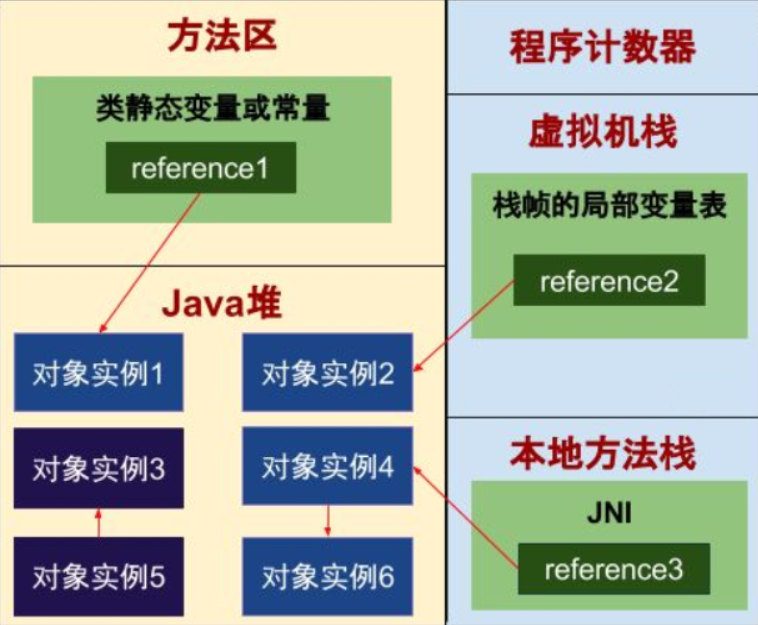
\includegraphics[scale=0.6]{./images/0001.png}
            \caption{Java Memory Model}
        \end{figure}
\end{enumerate}

\subsection{垃圾回收算法}
\subsubsection{标记-清除算法(Mark-Sweep)}
顾名思义,其分为“标记”和“清除”两个阶段:首先标记出所有需要回收的对象,标记完成后统一回收所有被标记的对象。这种算法的不足主要体现在效率和空间,从效率的角度讲,标记和清除两个过程的效率都不高;从空间的角度讲,标记清除后会产生大量不连续的内存碎片,内存碎片太多可能会导致以后程序运行过程中在需要分配较大对象时,无法找到足够的连续内存,而不得不提前触发一次垃圾收集动作,如图:
\begin{figure}[H]
    \centering
    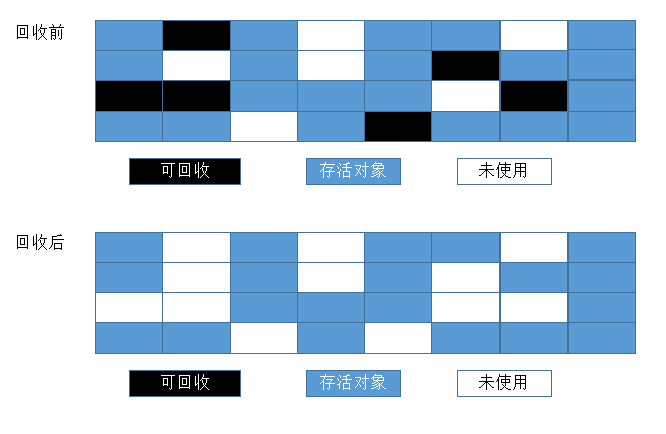
\includegraphics[scale=0.5]{./images/0008.png}
    \caption{Mark-Sweep GC}
\end{figure}
\subsubsection{复制算法(Copying)}
复制算法是为了解决效率问题而出现的,它将可用的内存分为两块,每次只用其中一块,当这一块内存用完了,就将还存活着的对象复制到另外一块上面,然后再把已经使用过的内存空间一次性清理掉。这样每次只需要对整个半区进行内存回收,内存分配时也不需要考虑内存碎片等复杂情况,只需要移动指针,按照顺序分配即可。复制算法的执行过程如图:
\begin{figure}[H]
    \centering
    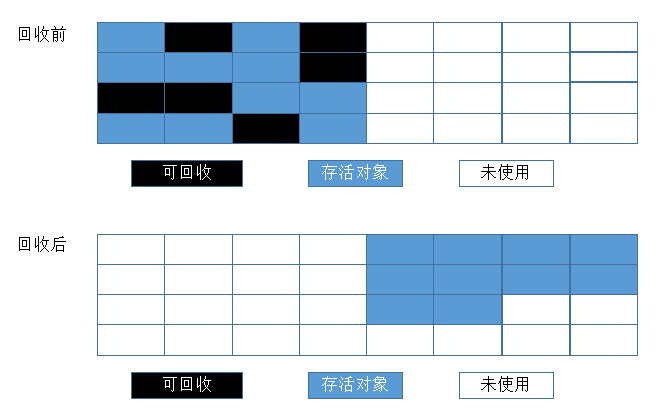
\includegraphics[scale=0.5]{./images/0009.png}
    \caption{Copying GC}
\end{figure}
\subsubsection{标记-整理算法(Mark-Compact)}
让所有存活对象都向一端移动,然后直接清理掉边界以外的内存。如图:
\begin{figure}[H]
    \centering
    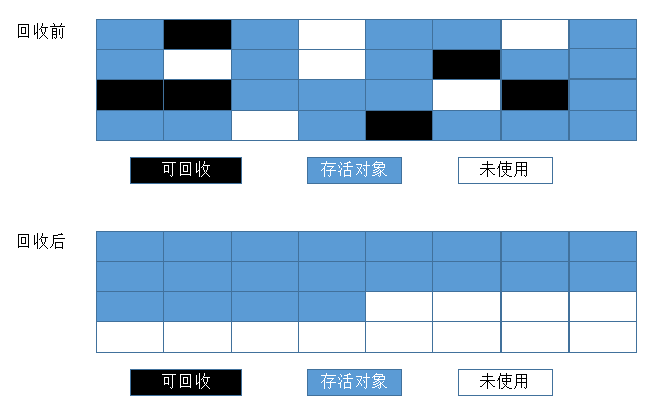
\includegraphics[scale=0.5]{./images/0010.png}
    \caption{Mark-Compact GC}
\end{figure}
\subsubsection{分代收集算法(Generational GC)}
分代收集算法将堆区分为如下几类:
\begin{figure}[H]
    \centering
    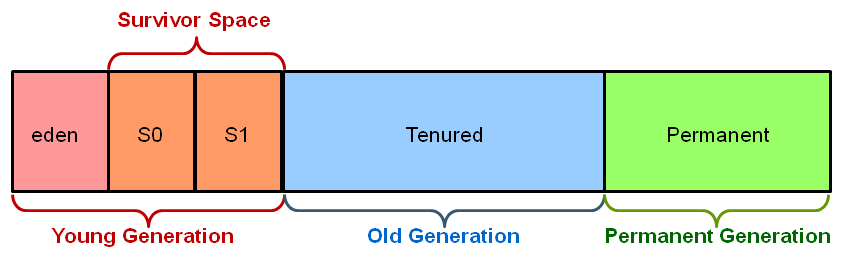
\includegraphics[scale=0.5]{./images/0002.png}
    \caption{Hotspot Heap Structure}
\end{figure}
\begin{enumerate}
    \item 新生代(Young Generation)
        \begin{enumerate}
            \item Eden Space(伊甸园):新对象分配内存的地方。
            \item Survivor Space(幸存者区):Survival区有两块survivor 0和survivor 1。
        \end{enumerate}
    \item 老年代(Tenured Generation):存放存活时间较久的,体积较大的对象。新生代与老年代的比例在1:2左右。
    \item 永久代(Permanent Generation):用于存放一些类的永久数据,JDK8之后不再有永久代。
\end{enumerate}
JVM的内存分配和回收过程如下:
\begin{enumerate}
    \item 所有的新对象都是在eden区进行分配的,两个survivor区在一开始都是空的:
        \begin{figure}[H]
            \centering
            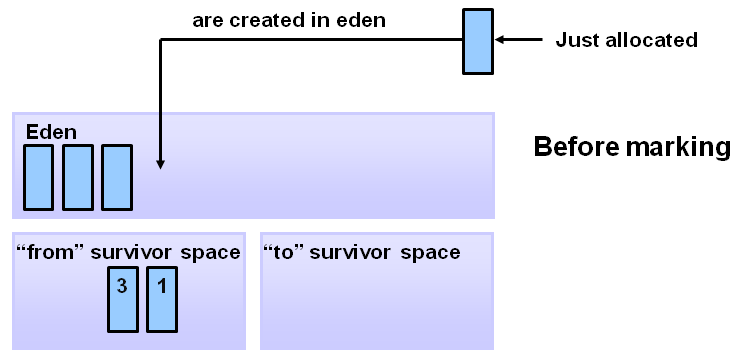
\includegraphics[scale=0.5]{./images/0003.png}
            \caption{Object Allocation}
        \end{figure}
    \item 当eden区满了之后,将会进行一次minor gc。
    \item minor gc时,经引用的对象都会被移动到survivor 0区,未收引用的对象(垃圾清除的目标)将会被直接删除:
        \begin{figure}[H]
            \centering
            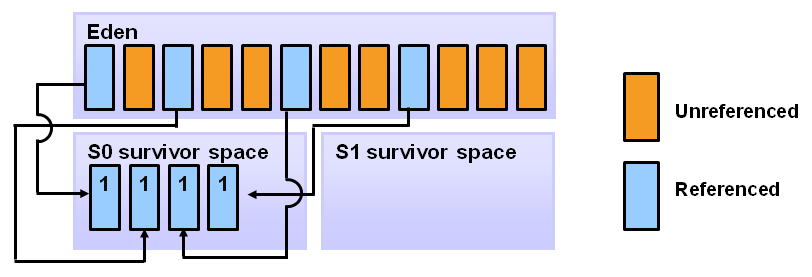
\includegraphics[scale=0.5]{./images/0004.png}
            \caption{Copying Referenced Objects}
        \end{figure}
    \item 再到下一次minor gc时,eden中经引用的对象将会被移动到survivor 1区,目前在survivor 0区的对象,经引用的,将引用计数+1,然后从survivor 0区移动到survivor 1区,未经引用的,将连同eden区一块进行内存释放。经由此过程后,survivor 1区内将会有2中不同年龄(引用计数)的对象:
        \begin{figure}[H]
            \centering
            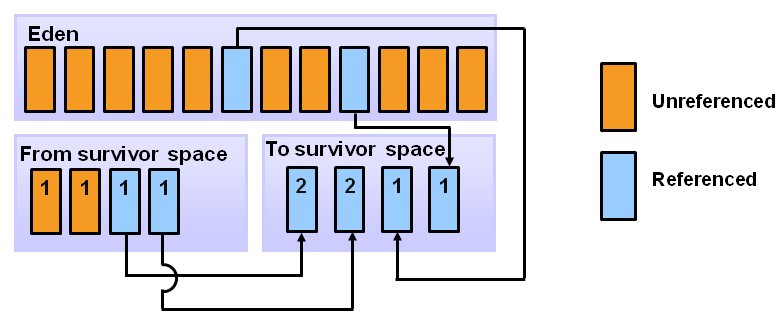
\includegraphics[scale=0.5]{./images/0005.png}
            \caption{Object Aging}
        \end{figure}
    \item 再到下一次minor gc时,eden区和survivor 1区中被引用的对象将会移动到survivor 0区(survivor区互换),然后移动的对象引用计数+1,eden区和survivor1区将会被回收:
        \begin{figure}[H]
            \centering
            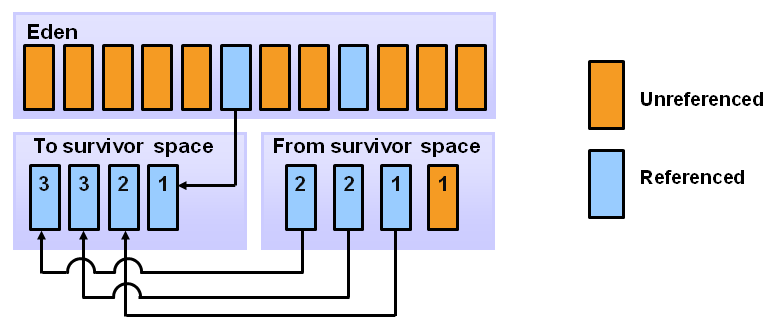
\includegraphics[scale=0.5]{./images/0006.png}
            \caption{Additional Aging}
        \end{figure}
    \item 经过一系列的minor gc之后,一些对象的引用计数将达到设定的阈值(例如8),这些足够老(达到阈值)的将会从新生代移动到老年代:
        \begin{figure}[H]
            \centering
            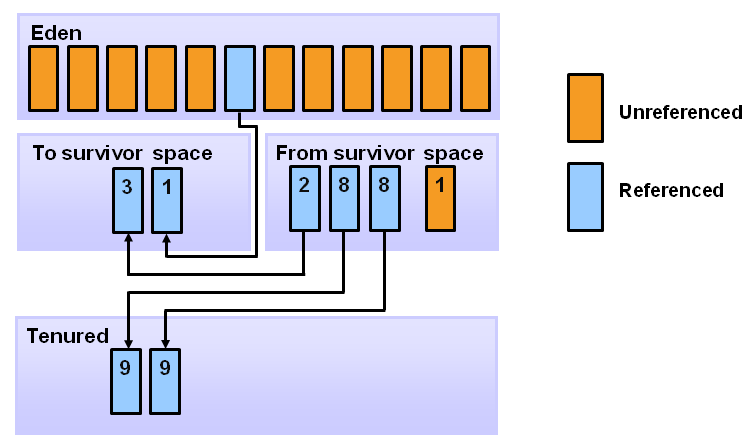
\includegraphics[scale=0.5]{./images/0007.png}
            \caption{Promotion}
        \end{figure}
    \item 当老年代满了之后,会触发major gc(full gc),major gc的发生频率较低,且老年代对象存活时间较长,存活标记率较高。
\end{enumerate}

\section{语言及语法相关}
\subsection{JDK和JRE的区别}
\begin{itemize}
    \item JDK是Java Development Kit,它是功能齐全的Java SDK。它拥有JRE所拥有的一切,还有编译器(javac)和工具(如javadoc和jdb),能够创建和编译程序。
    \item JRE 是Java运行时环境。用于运行已编译的Java程序,包括 Java虚拟机(JVM),Java类库,java命令和其他的一些基础构件,不能用于创建新程序。
\end{itemize}

\subsection{equals、hashCode和==}
==对于基本数据类型比较的是值,对于对象,比较的是对象的堆地址是否相等。Object类中equals()方法底层依赖的是==,默认的Object类中使用equals方法也是对比的对象的堆地址是否相等。hashCode是计算的对象的散列值。三者关系如下:
\begin{enumerate}
    \item 两个对象的hashcode相同,对象不一定是同一个对象。
    \item 两个对象的hashcode不同,那一定不是同一个对象。
    \item 如果两个对象的equals相同,那么hashcode一定相同。
\end{enumerate}
有关String对象的特殊说明,看下面的代码:\\
\begin{minted}{java}
    String a = "ab";
    String b = "ab";
    System.out.println(a == b);
    String c = "a";
    String d = c + "b";
    System.out.println(a == d);
\end{minted}
第一个输出为true,因为"ab"为字符串直接量,同样的字符串直接量将被存储为一个实例,所以a和b都指向一个实例,地址相同,==结果即为true。而a和d的地址不同,所以比较结果为false。而再看这段代码:\\
\begin{minted}{java}
    String a = "ab";
    String b = "ab";
    System.out.println(a.hashCode() == b.hashCode());
    String c = "a";
    String d = c + "b";
    System.out.println(a.hashCode() == d.hashCode());
\end{minted}
首先明确,String类的hashCode值是和其保存的字符串有直接关系的,相同的字符串将会有相同的hashCode值,所以上述代码中,两个地址均输出true。String类型的hashCode计算规则为:\\
\begin{minted}{java}
    s[0]*31^(n-1) + s[1]*31^(n-2) + ... + s[n-1]
\end{minted}

\subsection{泛型中的<? super T>和<? extends T>}
首先,<? super T>表示包括T在内的任何T的父类,<? extends T>表示包括T在内的任何T的子类。你不能往List<? extends T>中插入任何类型的对象,因为你不能保证列表实际指向的类型是什么,你并不能保证列表中实际存储什么类型的对象。唯一可以保证的是,你可以从中读取到T或者T的子类。相反,如果是super就可以写入,因为其基本原则就是,可以将子类的对象赋值给父类,而不可以将父类的对象赋值给子类。同时,List<? super T>往外取时只能放在Object对象里。

\subsection{PECS原则}
PECS即Producer Extends Consumer Super,换句话说,生产者(外界频繁读取数据的)使用<? extends T>,消费者使用<? super T>。简而言之就是:
\begin{enumerate}
    \item 如果你需要从集合中获取类型T,那就使用<? extends T>。
    \item 如果你需要将类型T放入集合中,那就使用<? super T>。
    \item 如果你既要获取又要放置元素,那就不使用任何通配符。
\end{enumerate}
例如在java.util.Collections中的集合复制的方法:
\begin{minted}{java}
    public static <T> void copy(List<? super T> dest, List<? extends T> src) {
        ...
    }
\end{minted}
复制源集合src,主要获得元素,所以用<? extends T>。复制目标集合dest,主要是设置元素,所以用<? super T>。

\subsection{抽象类和接口}
\begin{enumerate}
    \item 接口的方法默认是 public,所有方法在接口中不能有实现(Java 8 开始接口方法可以有默认实现),抽象类可以有非抽象的方法。
    \item 接口中的实例变量默认是 final 类型的,而抽象类中则不一定。
    \item 一个类可以实现多个接口,但最多只能继承一个抽象类。
    \item 一个类实现接口的话要实现接口的所有方法,而抽象类不一定。
    \item 在JDK8中,接口也可以定义静态方法,可以直接用接口名调用。
\end{enumerate}

\section{IO}
\subsection{BIO (同步阻塞IO)}
线程发起IO请求,不管内核是否做好IO准备,从发起请求起,线程一直阻塞,直到操作完成。其根本特性就是做完一件事再去做另一件事,一件事做之前一定要等到前一件事做完。如果线程在执行过程中依赖于需要等待的资源,那么该线程会长期处于阻塞状态,此时处理机就会进行线程的切换,如果在高并发的web或者tcp服务器中系统开辟成千上万的线程,那么处理机的时间就会浪费在线程的切换中,使得线程的执行效率大大降低。

\subsection{NIO (同步非阻塞IO)}
线程发起IO请求,立即返回,内核在做好IO操作准备后,通过调用注册的回调函数通知线程做IO操作,线程开始阻塞,直到操作完成。客户端发送的连接请求都会注册到多路复用器上,多路复用器轮询到连接有IO请求时才启动一个线程进行处理。NIO适用于连接数目较多且连接比较短的架构,比如聊天服务器。\\
NIO的最重要的地方是当一个连接创建后,不需要对应一个线程,这个连接会被注册到多路复用器上面,所以所有的连接只需要一个线程就可以搞定,当这个线程中的多路复用器进行轮询的时候,发现连接上有请求的话,才开启一个线程进行处理,也就是一个请求一个线程模式。

\subsection{AIO (异步非阻塞IO)}
异步非阻塞I/O,服务器实现模式为一个有效请求一个线程,客户端的IO请求都是由操作系统先完成了再通知服务器用其启动线程进行处理。对于读操作而言,当有流可读取时,操作系统会将可读的流传入read方法的缓冲区,并通知应用程序。对于写操作而言,当操作系统将write方法传递的流写入完毕时,操作系统主动通知应用程序。AIO相对于NIO的区别在于,NIO需要使用者线程不停的轮询IO对象,来确定是否有数据准备好可以读了,而AIO则是在数据准备好之后,才会通知数据使用者,这样使用者就不需要不停地轮询了。

\subsection{三者的适用场景}
\begin{enumerate}
    \item BIO:适用于连接数目比较小且固定的架构,对服务器资源要求比较高,并发局限于应用中,JDK1.4以前的唯一选择。
    \item NIO:适用于连接数目多且连接比较短(轻操作)的架构,比如聊天服务器,并发局限于应用中,编程比较复杂,JDK1.4开始支持。
    \item AIO:适用于连接数目多且连接比较长(重操作)的架构,比如相册服务器,充分调用OS参与并发操作,编程比较复杂,JDK7开始支持。
\end{enumerate}

\subsection{同步与异步的区别}
\begin{enumerate}
    \item 同步:发送一个请求,等待返回,再发送下一个请求,同步可以避免出现死锁,脏读的发生。
    \item 异步:发送一个请求,不等待返回,随时可以再发送下一个请求,可以提高效率,保证并发。
\end{enumerate}

\subsection{阻塞与非阻塞的区别}
\begin{enumerate}
    \item 阻塞调用是指调用结果返回之前,当前线程会被挂起,调用线程只有在得到结果之后才会返回。
    \item 非阻塞调用指在不能立刻得到结果之前,该调用不会阻塞当前线程。
\end{enumerate}

\section{Java集合框架}
\subsection{ArrayList和LinkedList的区别}
\begin{enumerate}
    \item 二者都不保证线程安全,但Vector保证线程安全。
    \item ArrayList底层是Object数组,LinkedList底层是双向链表。
    \item ArrayList插入和删除复杂度为O(n),而LinkedList为O(1)。
    \item ArrayList支持快速随机访问,LinkedList不支持。
\end{enumerate}

\subsection{HashMap和HashTable的区别}
\begin{enumerate}
    \item HashMap是非线程安全的,HashTable是线程安全的。也因此HashMap要比 HashTable效率高一点。
    \item HashMap中,null可以作为键,这样的键只有一个。HashTable不支持null作为键,否则抛出NullPointerException。
\end{enumerate}

\subsection{HashMap和HashSet的区别}
\begin{enumerate}
    \item HashSet底层基于HashMap实现。
    \item HashSet实现了Set接口,仅用来存储对象,而不是键值对。
    \item HashSet使用成员对象来计算hashCode值,而HashMap使用key。同步:发送一个请求,等待返回,再发送下一个请求,同步可以避免出现死锁,脏读的发生
    \item HashSet比HashMap慢。
\end{enumerate}

\subsection{HashMap的长度为什么是2的幂次方}
HashMap中的tableSizeFor()方法用来保证HashMap总是使用2的幂作为哈希表的大小。原因是因为经计算出来的hash值需要对数组长度进行取余运算,然后用余数定位其在hash表中的位置,为了优化取余运算的效率,人们发现取余(\%)操作中如果除数是2的幂次则等价于与其除数减一的与(\&)操作,及hash\%length等价于hash\&(length-1),前提是length是2的n次方,采用二进制位操作\&,相对于\%能够提高运算效率。

\subsection{HashMap多线程操作导致死循环问题}
多线程下对HashMap进行put操作会导致死循环问题,原因在于HashMap扩容使用的resize方法,由于扩容是新建一个数组,然后复制原数据到数组,由于数组下标挂有链表,所以需要复制链表,但多线程操作有可能导致环形链表,模拟过程如下:\\
假设当前HashMap的空间为2,hashCode分别为0和1,散列地址为0的地方有元素A和B,这个时候需要添加元素C,经过hash运算,元素C的散列地址为1,这时调用resize方法进行扩容,此时线程1读取到HashMap当前的情况,准备扩容:
\begin{figure}[H]
    \centering
    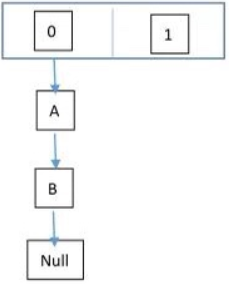
\includegraphics[scale=0.5]{./images/0013.png}
\end{figure}
然后线程2介入,读取HashMap进行扩容:
\begin{figure}[H]
    \centering
    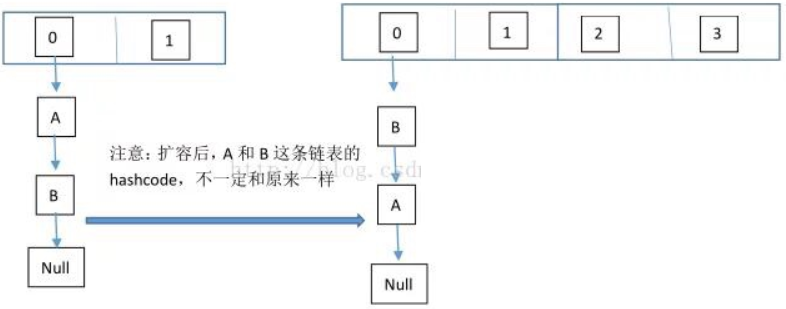
\includegraphics[scale=0.5]{./images/0014.png}
\end{figure}
此后线程1继续执行:
\begin{figure}[H]
    \centering
    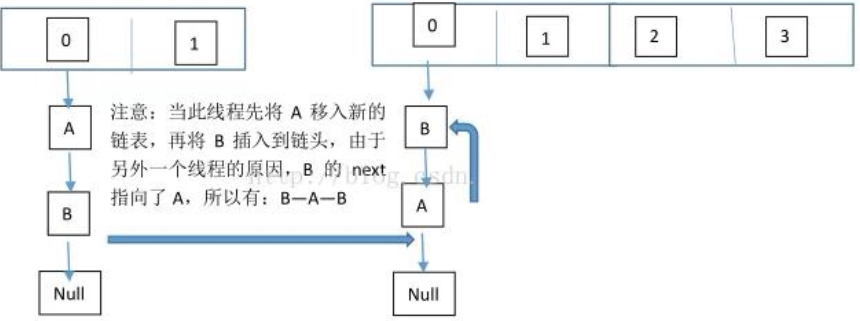
\includegraphics[scale=0.5]{./images/0015.png}
\end{figure}
这个过程为,先将A复制到新的hash表中,然后接着复制B到链表表头(A的前边,即B.next=A),本来 B.next=null,到此也就结束了,但是,由于线程二扩容的原因,将B.next=A,所以,这里继续复制A,让A.next=B,由此,环形链表出现:B.next=A; A.next=B。

\subsection{ConcurrentHashMap线程安全的具体实现方式}
\subsubsection{JDK 1.7}
\begin{figure}[H]
    \centering
    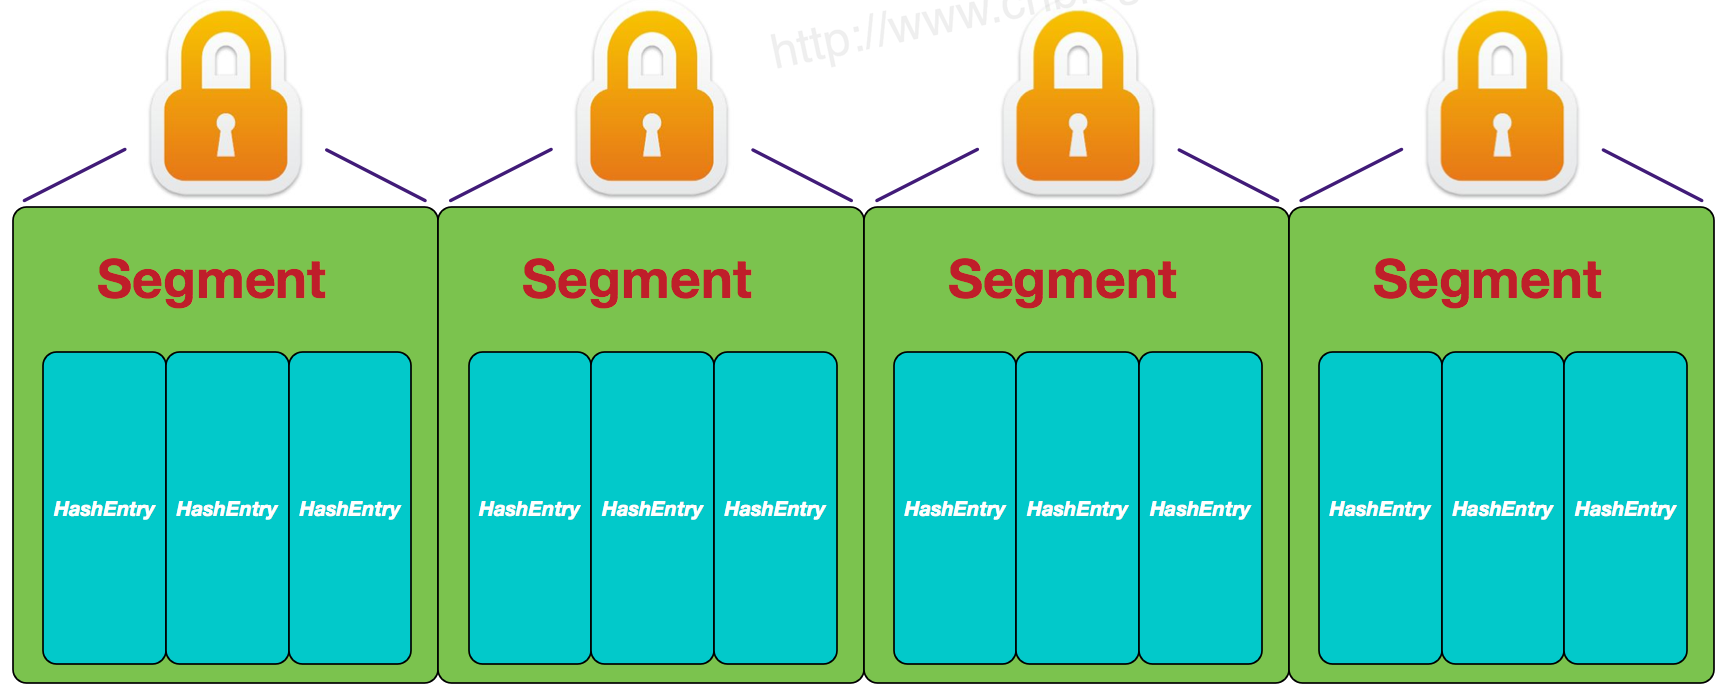
\includegraphics[scale=0.3]{./images/0011.png}
    \caption{ConcurrentHashMap 分段锁}
\end{figure}
使用分段锁来实现线程安全,将数据分为一段一段的存储,然后为每一段数据配一把锁,当一个线程访问占用锁访问一段数据时,其他段的数据也能被其他线程访问。一个ConcurrentHashMap里包含一个Segment数组。Segment的结构和HashMap类似,是一种数组加链表结构,一个Segment包含一个HashEntry数组,HashEntry用于存放键值对数据,每个HashEntry是一个链表结构的元素,每个Segment守护着一个HashEntry数组里的元素,当对HashEntry数组的数据进行修改时,必须首先获得对应的Segment的锁。
\subsubsection{JDK 1.8}
\begin{figure}[H]
    \centering
    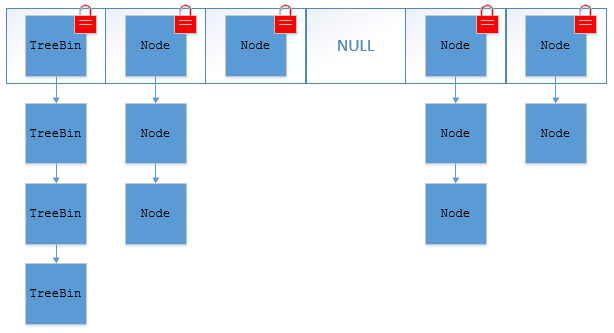
\includegraphics{./images/0012.png}
    \caption{ConcurrentHashMap 分段锁}
\end{figure}
JDK 1.8之后取消了分段锁,采用了synchronized来保证并发安全,synchronized只锁定当前链表或红黑树的首节点,这样只要hash不冲突,就不会产生并发问题。

\chapter{Spring}
\section{Spring AOP}
\subsection{描述一下Spring AOP及关注点和横切关注点}
AOP即面向切面编程,剖解开封装的对象内部,并将那些影响了多个类的公共行为封装到一个可重用模块,并将其名为“Aspect”,即切面。简单地说,就是将那些与业务无关,却为业务模块所共同调用的逻辑封装起来,便于减少系统的重复代码,降低模块间的耦合度,并有利于未来的可操作性和可维护性。Spring中AOP代理由Spring的IOC容器负责生成、管理,其依赖关系也由IOC容器负责管理。因此,AOP代理可以直接使用容器中的其它bean实例作为目标,这种关系可由IOC容器的依赖注入提供。AOP的关键单元是切面,或者说关注点,即为我们想实现特定业务功能的方法。一些切面可能有集中的代码,但是有些可能被分散或者混杂在一起,例如日志或者事务。这些分散的切面被称为横切关注点。横切关注点是贯穿整个应用程序的关注点。像日志、安全和数据转换。\\
AOP的最大意义其实就是在不改变原来代码的前提下,也不对源代码做任何协议接口要求。而实现了类似插件的方式,来修改源代码,给源代码插入新的执行代码。
\subsection{Spring中有哪些不同的通知类型}
通知(advice)是切面的具体逻辑实现。有以下5种形式:
\begin{enumerate}
    \item 前置通知(Before Advice):在连接点之前执行的Advice,不过除非它抛出异常,否则没有能力中断执行流。使用@Before注解使用这个Advice。
    \item 返回后通知(After Retuning Advice):在连接点正常结束之后执行的Advice。例如一个方法没有抛出异常并正常返回。通过@AfterReturning注解来使用。
    \item 抛出(异常)后执行通知(After Throwing Advice):如果一个方法通过抛出异常来退出的话,这个Advice就会被执行。通过@AfterThrowing注解来使用。
    \item 后置通知(After Advice):无论连接点是通过什么方式退出的(正常返回或者抛出异常)都会执行在结束后执行这些Advice。通过@After注解使用。
    \item 环绕通知(Around Advice):决定是否调用目标方法,而且能够获得到目标方法的返回值,而且还能改变这些返回值。通过@Around注解使用。
\end{enumerate}
\subsection{代理模式}
代理模式给某一个对象提供一个代理对象,并由代理对象控制对原对象的引用。其主要特点是在不改变原有类的前提下,在原有类某些方法执行前后,插入执行任意代码。所以代理模式需要写新的类对原有的类进行包装,有如下三种实现方式:
\subsubsection{静态代理}
需要增强原有类的哪个方法,就需要对在代理类中包装哪个方法。在使用时,需要定义接口或者父类,被代理对象与代理对象一起实现相同的接口或者是继承相同父类。例如:\\
接口IUserDao.java
\begin{minted}{java}
    public interface IUserDao {
        void save();
    }
\end{minted}
需要代理的目标对象UserDao.java
\begin{minted}{java}
    public class UserDao implements IUserDao {
        public void save() {
            System.out.println("---- Already saved!----");
        }
    }
\end{minted}
代理对象UserDaoProxy.java
\begin{minted}{java}
    public class UserDaoProxy implements IUserDao {
        // the object needed to be proxied
        private IUserDao target;

        public UserDaoProxy(IUserDao target){
            this.target=target;
        }

        public void save() {
            System.out.println("Start transaction");
            target.save(); // the target method
            System.out.println("Commit transaction");
        }
    }
\end{minted}
测试类App.java
\begin{minted}{java}
    public class App {
        public static void main(String[] args) {
            UserDao target = new UserDao();
            // proxy object
            UserDaoProxy proxy = new UserDaoProxy(target);
            proxy.save();
        }
    }
\end{minted}
静态代理的缺点是代理对象需要与目标对象实现一样的接口,所以会产生很多代理类,为日后的维护增添麻烦。
\subsubsection{动态代理}
动态代理利用反射机制,对象和方法都是传入的变量,以此动态调用被代理对象的任何方法,JDK实现代理,只需要使用newProxyInstance方法,还是上面的那个例子,只不过我们这次用动态代理机制来将其实现一下:\\
代理工厂类ProxyFactory.java
\begin{minted}{java}
    public class ProxyFactory {
        // the object which needed to be proxied
        private Object target;

        public ProxyFactory(Object target){
            this.target=target;
        }

        // generate proxy instance
        public Object getProxyInstance(){
            // invoke newProxyInstance method
            return Proxy.newProxyInstance(
                    target.getClass().getClassLoader(),
                    target.getClass().getInterfaces(),
                    new InvocationHandler() {
                        @Override
                        public Object invoke(Object proxy, Method method, Object[] args) throws Throwable {
                            System.out.println("Start transaction");
                            // invoke target object method and get return value
                            Object returnValue = method.invoke(target, args);
                            System.out.println("Commit transaction");
                            return returnValue;
                        }
                    }
            );
        }
    }
\end{minted}
测试类App.java
\begin{minted}{java}
    public class App {
        public static void main(String[] args) {
            // original object
            IUserDao target = new UserDao();
            System.out.println(target.getClass());

            // get a proxy instance for target object
            IUserDao proxy = (IUserDao) new ProxyFactory(target).getProxyInstance();
            System.out.println(proxy.getClass());

            // invoke method
            proxy.save();
        }
    }
\end{minted}
\subsubsection{CGLIB代理}
静态代理和动态代理都要求目标对象是实现一个特定接口的目标对象,但有的时候一个对象是一个单独的对象,并没有实现任何接口,这个时候就可以使用以目标对象子类的方式类实现代理,即CGLIB代理,也叫做子类代理。显然,代理的类不能被标记为final,否则报错。\\
使用CGLIB代理时需要引入cglib的jar文件,如果你用了Spring,其核心中已经包括了这个包,所以可以直接引入包spring-core,代码实例:\\
没有实现任何接口的目标对象类UserDao.java
\begin{minted}{java}
    public class UserDao {
        public void save() {
            System.out.println("----已经保存数据!----");
        }
    }
\end{minted}
CGLIB代理工厂ProxyFactory.java
\begin{minted}{java}
    public class ProxyFactory implements MethodInterceptor {
        // the target object needed to be proxied
        private Object target;

        public ProxyFactory(Object target) {
            this.target = target;
        }

        // create a proxy object instance
        public Object getProxyInstance(){
            // tool instance
            Enhancer en = new Enhancer();
            // set super class of CGLIB proxy
            en.setSuperclass(target.getClass());
            en.setCallback(this);
            // create proxy instance
            return en.create();
        }

        @Override
        public Object intercept(Object obj, Method method, Object[] args, MethodProxy proxy) throws Throwable {
            System.out.println("Start transaction");
            // invoke the super class method
            Object returnValue = method.invoke(target, args);
            System.out.println("Commit transaction");
            return returnValue;
        }
    }
\end{minted}
测试类App.java
\begin{minted}{java}
    public class App {
        @Test
        public void test(){
            UserDao target = new UserDao();
            UserDao proxy = (UserDao) new ProxyFactory(target).getProxyInstance();
            proxy.save();
        }
    }
\end{minted}

\section{Spring IOC}
\subsection{IOC的基本思想}
IOC即Inversion of Control,控制反转。通常,每个对象在使用他的合作对象时,自己需要使用像new Object()这样的语句来完成合作对象的申请工作。这样会造成对象间的耦合度高。IOC的思想是:Spring容器来实现这些相互依赖对象的创建、协调工作。对象只需要关系业务逻辑本身就可以了。从这方面来说,对象如何得到他的协作对象的责任被反转了(IOC、DI)。\\
Spring所倡导的开发方式就是如此:所有的类都会在spring容器中登记,告诉spring你是个什么东西,你需要什么东西,然后spring会在系统运行到适当的时候,把你要的东西主动给你,同时也把你交给其他需要你的东西。所有的类的创建、销毁都由spring来控制,也就是说控制对象生存周期的不再是引用它的对象,而是spring。对于某个具体的对象而言,以前是它控制其他对象,现在是所有对象都被spring控制,所以这叫控制反转。
\subsection{依赖注入DI}
IoC的一个任务是在系统运行中,动态的向某个对象提供它所需要的其他对象。这一点是通过DI(Dependency Injection,依赖注入)来实现的。比如对象A需要操作数据库,以前我们总是要在A中自己编写代码来获得一个Connection对象,有了 spring我们就只需要告诉spring,A中需要一个Connection,至于这个Connection怎么构造,何时构造,A不需要知道。A需要依赖Connection才能正常运行,而这个Connection是由spring注入到A中的,这即为依赖注入。

\section{Spring Bean}
\subsection{bean的作用域}
bean一共有如下5种作用域:
\begin{enumerate}
    \item singleton(单例):在IoC容器中仅存在一个bean实例,以单例的形式存在,默认值。
    \item prototype(原型):每次请求都会创建一个新的bean实例,即每次调用getBean()时,相当于执行new XXBean()。
    \item request:每次HTTP请求都会创建一个新的bean,该bean仅在当前HTTP request内有效,该作用域仅适用于WebApplicationContext环境。
    \item session:每一次HTTP请求都会产生一个新的bean,该bean仅在当前HTTP session内有效,仅适用于WebApplicationContext环境。
    \item global-session:所有的session共享一个bean实例
\end{enumerate}
设置bean的作用域:\\
\begin{minted}{xml}
    <bean id="..." class="..." scope="singleton">
        ...
    </bean>
\end{minted}
在xml中我们可以使用属性lazy-init=“true”来延迟加载bean,这样,只有在第一次获取bean时,才会初始化bean,或者使用注解的形式:\\
\begin{minted}{java}
    @Service
    @Scope("singleton")
    public class ServiceImpl{

    }
\end{minted}

\subsection{bean的加载}
\begin{figure}[H]
    \centering
    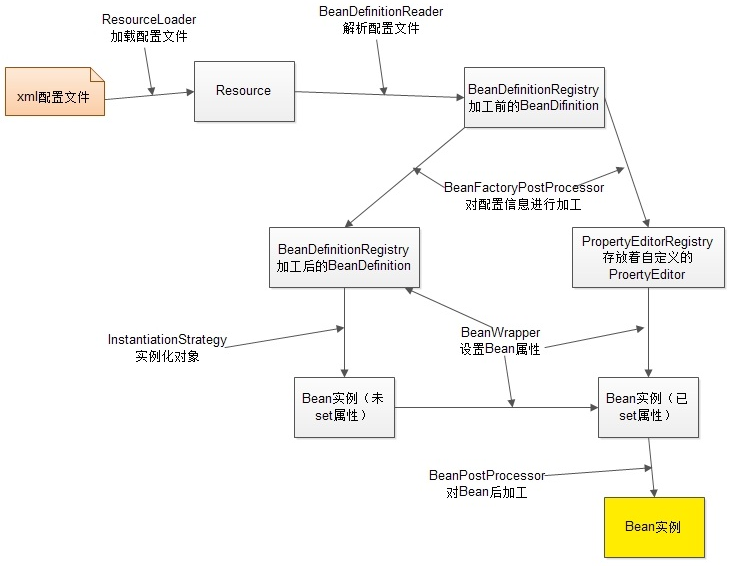
\includegraphics[scale=0.75]{./images/0018.png}
    \caption{bean的加载流程}
\end{figure}
\begin{enumerate}
    \item ResourceLoader从XML中加载Spring配置信息,并使用Resource表示这个配置文件的资源。
    \item BeanDefinitionReader读取Resource所指向的配置文件资源,然后解析配置文件。配置文件中每一个<bean>解析成一个BeanDefinition对象,并保存到BeanDefinitionRegistry中。
    \item 容器扫描BeanDefinitionRegistry中的BeanDefinition,使用Java的反射机制自动识别出实现了Bean工厂后处理器接口(BeanFactoryPostProcessor)的Bean,然后调用这些Bean工厂后处理器对BeanDefinitionRegistry中的BeanDefinition进行加工处理。在此过程中主要完成如下两项工作:
        \begin{enumerate}
            \item 对使用占位符<bean>的标签进行解析得到最终的配置值
            \item 对BeanDefinitionRegistry中的BeanDefinition进行扫描,通过反射机制找出所有实现了java.beans.PropertyEditor接口的Bean,然后将其注册到Spring容器的属性编辑器注册表中(PropertyEditorRegistry)。
        \end{enumerate}
    \item Spring容器从BeanDefinitionRegistry中取出加工后的BeanDefinition,并调用InstantiationStrategy着手进行Bean实例化的工作。
    \item 在实例化Bean时,Spring容器使用BeanWrapper对Bean进行封装,BeanWrapper通过反射机制操作Bean中的方法,结合该Bean的BeanDefinition以及容器中属性编辑器,完成Bean属性的设置工作。
    \item 利用容器中注册的Bean后处理器(实现BeanPostProcessor接口的Bean)对已经完成属性设置工作的Bean进行后续加工,直接装配出一个准备就绪的Bean。
\end{enumerate}

\section{Spring MVC}
\subsection{Spring MVC的工作流程}
客户端发送请求 -> 前端控制器DispatcherServlet接受客户端请求 -> 找到处理器映射HandlerMapping解析请求对应的Handler -> HandlerAdapter会根据Handler来调用真正的处理器开始处理请求,并处理相应的业务逻辑 -> 处理器返回一个模型视图ModelAndView -> 视图解析器进行解析 -> 返回一个视图对象 -> 前端控制器DispatcherServlet渲染数据(Moder) -> 将得到视图对象返回给用户。
\begin{figure}[H]
    \centering
    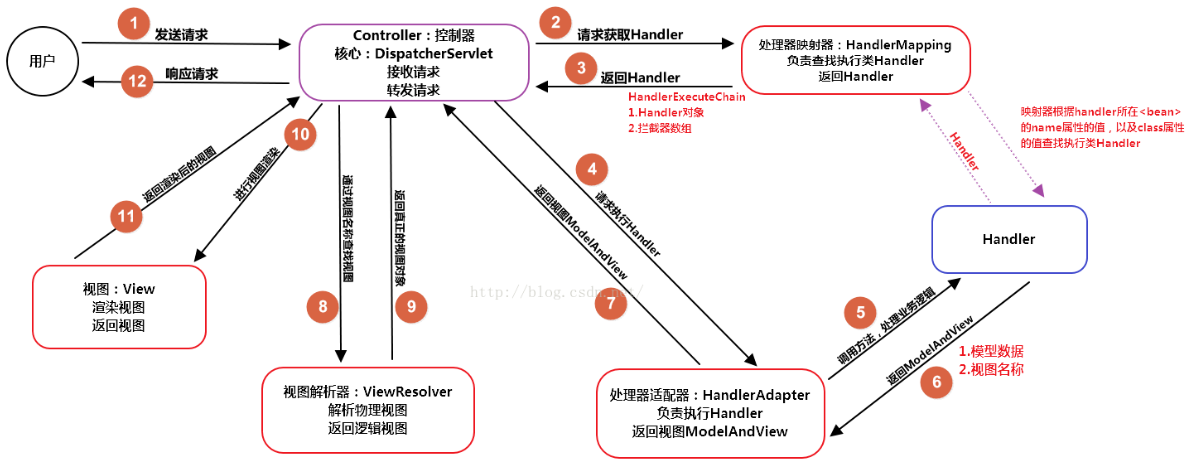
\includegraphics[scale=0.65]{./images/0016.png}
    \caption{Spring MVC工作流程}
\end{figure}
\subsection{SpringMVC怎么样设定重定向和转发的}
在返回值前面加"forward:"就可以让结果转发,譬如"forward:user.do?name=method4"\\
在返回值前面加"redirect:"就可以让返回值重定向,譬如"redirect:http://www.baidu.com"

\chapter{MySQL and MyBatis}
\section{事务}
\subsection{事务的ACID特性}
事务就是被绑定在一起作为一个逻辑工作单元的 SQL 语句分组,如果其中一个语句操作失败那么整个操作就被失败,以后操作就会回滚到操作前状态。事务具有ACID四大特性:
\begin{enumerate}
    \item 原子性(Atomicity):事务是最小的执行单位,不允许分割。事务的原子性确保动作要么全部完成,要么完全不起作用。
    \item 一致性(Consistency):执行事务前后,数据库从一个一致性状态转换到另一个一致性状态。
    \item 隔离性(Isolation):并发访问数据库时,一个用户的事物不被其他事务所干扰,各并发事务之间数据库是独立的。
    \item 持久性(Durability):一个事务被提交之后。它对数据库中数据的改变是持久的,即使数据库发生故障也不应该对其有任何影响。
\end{enumerate}

\subsection{并发事务带来的问题}
\begin{enumerate}
    \item 脏读(Dirty read):当一个事务正在访问数据并且对数据进行了修改,而这种修改还没有提交到数据库中,这时另外一个事务也访问了这个数据,然后使用了这个数据。因为这个数据是还没有提交的数据,那么另外一个事务读到的这个数据是“脏数据”,依据“脏数据”所做的操作可能是不正确的。
    \item 丢失修改(Lost to modify):在一个事务读取一个数据时,另外一个事务也访问了该数据,那么在第一个事务中修改了这个数据后,第二个事务也修改了这个数据。这样第一个事务内的修改结果就被丢失,因此称为丢失修改。
    \item 不可重复读(Unrepeatable read):指在一个事务内多次读取同一数据。在这个事务还没有结束时,另一个事务也访问该数据。那么,在第一个事务中的两次读数据之间,由于第二个事务的修改导致第一个事务两次读取的数据可能不一样。这就发生了在一个事务内两次读到的数据是不一样的情况,因此称为不可重复读。
    \item 幻读(Phantom read):第一个事务读取了几行数据,接着另一个并发事务插入了一些数据,在随后第一个事务的读取中,就会发现多了一些原本不存在的记录,就像发生了幻觉一样,因此称为幻读。例如:某工资单表中工资大于3000的有4人,事务1读取了所有工资大于3000的人,共查到4条记录,这时事务2又插入了一条工资大于3000的记录,事务1再次读取时查到的记录就变为了5条,这样就导致了幻读。
\end{enumerate}

\subsection{事务的隔离级别}
\begin{enumerate}
    \item READ\_UNCOMMITTED(未提交读):最低的隔离级别,允许读取尚未提交的数据变更,可能会导致脏读、幻读或不可重复读。
    \item READ\_COMMITTED(提交读):允许读取并发事务已经提交的数据,可以阻止脏读,但是幻读或不可重复读仍有可能发生。
    \item REPEATABLE\_READ(可重复读):对同一字段的多次读取结果都是一致的,除非数据是被本身事务自己所修改,可以阻止脏读和不可重复读,但幻读仍有可能发生。
    \item SERIALIZABLE(串行):最高的隔离级别,完全服从ACID的隔离级别。所有的事务依次逐个执行,这样事务之间就完全不可能产生干扰,也就是说,该级别可以防止脏读、不可重复读以及幻读。但是这将严重影响程序的性能。
\end{enumerate}
此处需注意:Mysql默认采用的REPEATABLE\_READ(可重复读)隔离级别,而Oracle默认采用的READ\_COMMITTED(未提交读)隔离级别。

\section{索引}
\subsection{索引的优缺点}
\subsubsection{优点}
\begin{enumerate}
    \item 大大加快数据检索的速度。
    \item 可以创建唯一性索引,保证数据库每一行的唯一性。
    \item 加速表与表之间的链接,特别是在实现数据的参考完整性方面特别有意义。
    \item 帮助服务器避免排序和临时表。
\end{enumerate}
\subsubsection{缺点}
\begin{enumerate}
    \item 需要占据一定的物理空间。
    \item 对表中的数据进行增加、删除和修改的时候,索引也要动态地维护,这就降低了数据的维护速度。
    \item 创建索引也需要耗费时间,而且所费时间与数据集的大小成正比。
\end{enumerate}

\subsection{索引的使用}
\subsubsection{应该在这些列上创建索引}
\begin{enumerate}
    \item 经常需要搜索的列上,可以加快搜索的速度。
    \item 经常使用WHERE子句的列上,可以加快条件判断的速度。
    \item 经常需要排序的列上,因为索引已经排序,故可以加快排序时间。
    \item 对于中到大型表,特大型表的索引维护开销会很大。
\end{enumerate}
\subsubsection{注意}
\begin{enumerate}
    \item 避免在WHERE子句中对字段施加函数,这会导致无法命中索引。
    \item 在InnoDB中使用与业务无关的自增主键,即使用逻辑主键而不是业务主键。
    \item 将打算索引的表设为NOT NULL,否则将导致引擎放弃索引而进行全表扫描。
    \item 可以通过删除长期未使用的索引来避免一些不必要的性能损耗。
    \item 索引可以提高limit子句的查询性能。
\end{enumerate}

\subsection{索引的数据结构}
\begin{enumerate}
    \item 哈希索引:底层数据结构为哈希表,如果绝大多数需求为查询单条记录可以选择hash索引,查询性能最快,其他场景建议选择BTree索引。
    \item BTree索引:MySQL的实现中底层数据结构为B+树
        \begin{enumerate}
            \item MyISAM引擎:索引文件与数据文件分离,B+树的叶节点data域存放数据记录的地址,在索引检索的时候,首先按B+树的搜索算法搜索索引,如果指定的key存在,则取出其data域的值,然后以data域的值为地址读取对应的数据记录,此方法被称为“非聚簇索引”。
            \item InnoDB引擎:其数据文件本身就是索引文件,其表数据文件本身就是按照B+树进行组织的一个索引结构,树节点的data域保存了完整的数据记录,这个索引的key就是数据表的主键,数据文件本身就是主索引,这被称为“聚簇索引”。而其余的索引都作为辅助索引,辅助索引的data域存储相对应记录主键的值而不是地址。所以,根据辅助索引查找时,先找到其主键的值,然后再走一遍主索引,找到整个字段。因此设计表时,不建议使用过长的字段作为主键,也不建议使用非单调的字段作为主键,这会造成主索引的频繁分裂。
        \end{enumerate}
\end{enumerate}

\subsection{覆盖索引}
如果一个索引包含所有需要查询的字段的值,我们就称之为“覆盖索引”。在InnoDB存储引擎中,如果不是主键索引,叶子结点存储的是主键+列值,最终还是要通过主键回表。这样就会比较慢,覆盖索引就不需要进行回表操作。

\subsection{索引查询的3个原则}
\begin{enumerate}
    \item 单行访问是很慢的,如果服务器从存储中读取一个数据块只是为了获取其中一行,那么就浪费了很多工作,最好读取的块中能包含尽可能多的所需要的行,使用索引可以创建位置索引,以提升效率。
    \item 按顺序访问范围数据时很快的,一是因为顺序IO不需要多次磁盘寻道,二是如果服务器能够按需要允许读取数据,就不需要额外的排序操作,使用GROUP BY的查询也无须排序和按组进行聚合计算。
    \item 覆盖索引查询是很快的,如果一个索引包含了查询所需的所有的列,那么存储引擎就不需要再回表按行查找了,这避免了大量的单行访问。
\end{enumerate}

\subsection{最左前缀原则}
MySQL中的索引可以以一定顺序引用多列,这种索引叫作联合索引。如User表的name和city加联合索引就是(name,city),而最左前缀原则指的是,如果查询的时候查询条件精确匹配索引的左边连续一列或几列,则此列就可以被用到。如下:
\begin{minted}{sql}
    select * from user where name=xx and city=xx; // 可以命中索引
    select * from user where name=xx; // 可以命中索引
    select * from user where city=xx; // 无法命中索引
\end{minted}
如果查询时两个条件都用上了,但是顺序不同,查询引擎会自动优化以匹配联合索引的顺序,也是可以命中索引的。

\section{数据库存储引擎}
\subsection{MyISAM和InnoDB的对比}
\begin{enumerate}
    \item count运算:MyISAM缓存有表meta-data(其中包含行数等),因此在做COUNT(*)时对于一个结构很好的查询是不需要消耗多少资源的。而对于InnoDB来说,则没有这种缓存。
    \item MyISAM强调的是性能,每次查询具有原子性,其执行速度比InnoDB更快,但是不提供事务支持。InnoDB支持事务,外部键等高级数据库功能。
    \item MyISAM不支持外键而InnoDB支持。
    \item MyISAM更适合读密集的表,而InnoDB更适合写密集的的表,在数据库做主从分离的情况下,经常选择MyISAM作为从库的存储引擎。
    \item MyISAM支持全文类型索引而InnoDB不支持。
\end{enumerate}

\section{锁机制}
\subsection{MyISAM和InnoDB存储引擎使用的锁}
\begin{enumerate}
    \item MyISAM采用表级锁(table-level locking)。InnoDB的锁是逐步获得的同时MyISAM总是一次性获得所需的全部锁。
    \item InnoDB支持行级锁(row-level locking)和表级锁,默认为行级锁。InnoDB的锁是逐步获得的,当两个事务都需要获得对方持有的锁,导致双方都在等待,这就产生了死锁。发生死锁后,InnoDB一般都可以检测到,并使一个事务释放锁回退,另一个则可以获取锁完成事务。
\end{enumerate}

\subsection{表级锁和行级锁对比}
\begin{enumerate}
    \item 表级锁:Mysql中锁定粒度最大的一种锁,对当前操作的整张表加锁,实现简单,资源消耗也比较少,加锁快,不会出现死锁。其锁定粒度最大,触发锁冲突的概率最高,并发度最低,MyISAM和 InnoDB引擎都支持表级锁。
    \item 行级锁:Mysql中锁定粒度最小的一种锁,只针对当前操作的行进行加锁。行级锁能大大减少数据库操作的冲突。其加锁粒度最小,并发度高,但加锁的开销也最大,加锁慢,会出现死锁。
    \item 页级锁:MySQL中锁定粒度介于行级锁和表级锁中间的一种锁。表级锁速度快,但冲突多,行级冲突少,但速度慢。页级进行了折衷,一次锁定相邻的一组记录。开销和加锁时间界于表锁和行锁之间,会出现死锁。锁定粒度界于表锁和行锁之间,并发度一般。
\end{enumerate}

\section{MyBatis}
\subsection{\#\{\}和\$\{\}的区别是什么}
\#\{\}是预编译处理,\$\{\}是字符串替换。MyBatis在处理\#\{\}时,会将sql中的\#\{\}替换为?号,调用PreparedStatement的set方法来赋值。MyBatis在处理\$\{\}时,会直接把\$\{\}替换成变量的值。使用\#\{\}可以有效的防止SQL注入,提高系统安全性。

\subsection{实体类中的属性名和表中的字段名不一样怎么办}
第一种可以在查询的sql语句中定义字段名的别名,让字段名的别名和实体类的属性名一致:
\begin{minted}{xml}
    <select id=”selectorder” parametertype=”int” resultetype=”me.gacl.domain.order”>
       select order_id as id, order_no as orderno ,order_price as price form orders where order_id=#{id};
    </select>
\end{minted}
第二种可以通过<resultMap>来映射字段名和实体类属性名的一一对应的关系:
\begin{minted}{xml}
    <select id="getOrder" parameterType="int" resultMap="orderresultmap">
        select * from orders where order_id=#{id}
    </select>

    <resultMap type=”me.gacl.domain.order” id=”orderresultmap”>
        <!– 用id属性来映射主键字段 –>
        <id property=”id” column=”order_id”>
        <!–用result属性来映射非主键字段–>
        <result property = “orderno” column =”order_no”/>
        <result property=”price” column=”order_price” />
    </reslutMap>
\end{minted}

\subsection{DAO接口的工作原理}
Dao接口的工作原理是JDK动态代理,MyBatis运行时会使用JDK动态代理为Dao接口生成代理proxy对象,代理对象proxy会拦截接口方法,转而执行MappedStatement所代表的sql,然后将sql执行结果返回。

\subsection{MyBatis是如何进行分页的}
MyBatis使用RowBounds对象进行分页,它是针对ResultSet结果集执行的内存分页,而非物理分页,可以在sql内直接书写带有物理分页的参数来完成物理分页功能,也可以使用分页插件来完成物理分页。分页插件的基本原理是使用MyBatis提供的插件接口,实现自定义插件,在插件的拦截方法内拦截待执行的sql,然后重写sql,添加对应的物理分页语句和物理分页参数。

\subsection{MyBatis的执行流程}
\begin{enumerate}
    \item 加载配置文件并初始化SqlSession。
    \item 接收调用请求,调用mybatis提供的api,传入的参数为sql的id(有namespase和具体sql的id组成)和sql语句的参数对象,mybatis将调用请求交给请求处理层。
    \item 根据sql的id找到对应的mapped statament对象。然后根据传入参数解析此对象,得到最终要执行的sql。
    \item 获取数据库连接,执行sql,得到执行结果。
    \item mapped statement对象中的结果映射对执行结果进行转换处理,并得到最终的处理结果。
\end{enumerate}
大致如图:
\begin{figure}[H]
    \centering
    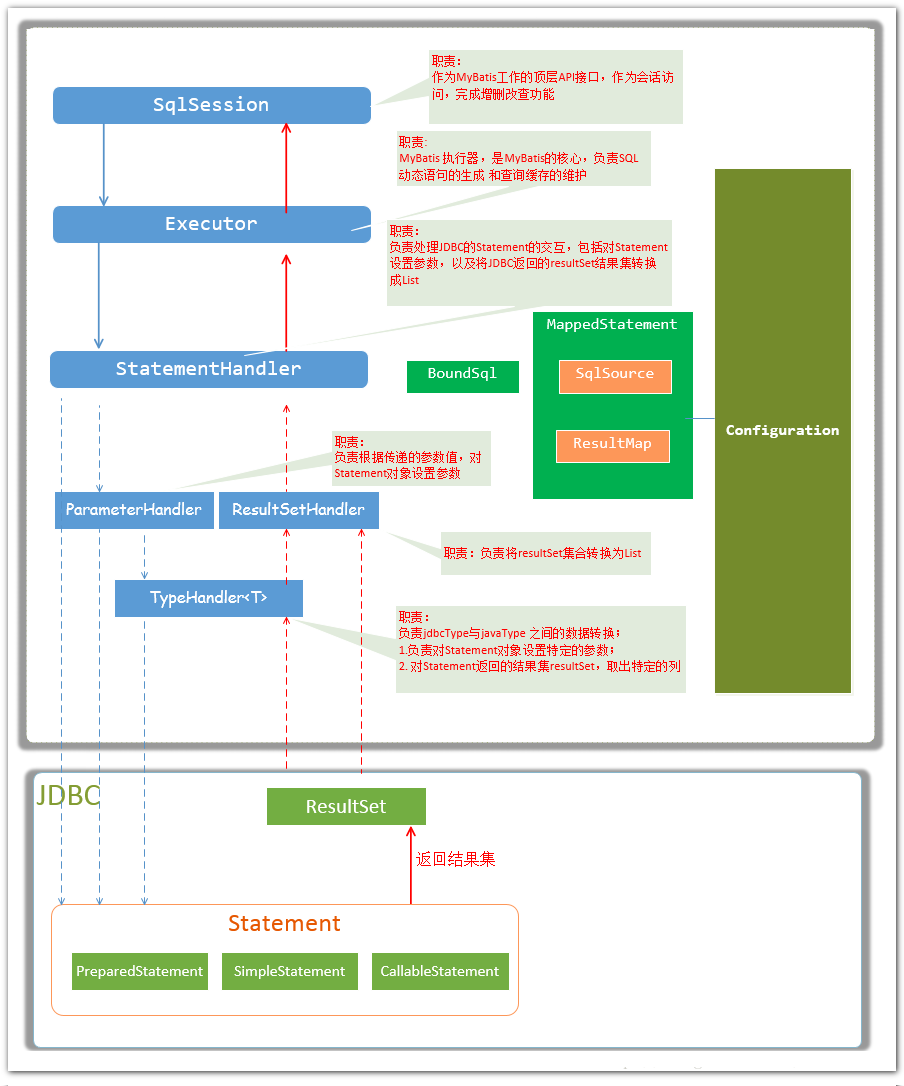
\includegraphics[scale=0.4]{./images/0017.png}
    \caption{MyBatis中SQL语句的执行流程}
\end{figure}

\subsection{MyBatis缓存}
\subsubsection{一级缓存}
一级缓存是sqlSession级别的缓存。在操作数据库时需要构造sqlSession对象,在对象中有一个HashMap用于存储缓存数据。不同的sqlSession之间的缓存数据区域是互不影响相互独立的。也就是他只能作用在同一个sqlSession中,不同的sqlSession中的缓存是互相不能读取的。Mybatis一级缓存默认开启。\\
这个HashMap的key是以查询的sql语句为基础的拼接出的一个字符串组成的。\\
用户发起查询请求,查找某条数据,sqlSession先去缓存中查找,是否有该数据,如果有从缓存中读取。如果没有,从数据库中查询,并将查询到的数据放入一级缓存,供下次查找使用。当sqlSession执行了commit操作(增删改),一级缓存会清空,以使得缓存的都是最新的数据,避免脏读。\\
如果commit不清空缓存,会有以下场景:A查询了某商品库存为10件,并将10件库存的数据存入缓存中,之后被客户买走了10件,数据被delete了,但是下次查询这件商品时,并不从数据库中查询,而是从缓存中查询,就会出现错误。\\
实际应用中,如果将Spring和Mybatis进行整合,事务控制发生在service中。service开始执行时创建sqlSession对象,结束时关闭sqlSession,如果刚刚产生了一级缓存的话,也会随着sqlSession而销毁。所以两次调用相同的service查询相同的信息,不会走一级缓存的。
\subsubsection{二级缓存}
二级缓存默认不开启。需要在MyBatis的配置文件中加入:
\begin{minted}{xml}
    <settings>
        <!-- 开启二级缓存 -->
        <setting name="cacheEnabled" value="true"/>
    </settings>
\end{minted}
以及在需要打开二级缓存的mapper.xml文件中加入cache标签:
\begin{minted}{xml}
    <cache/>
\end{minted}
同时也要让使用二级缓存的POJO类实现Serializable接口,例如:
\begin{minted}{java}
    public class User implements Serializable {
        ...
    }
\end{minted}
二级缓存是mapper级别的缓存,多个SqlSession去操作同一个Mapper的sql语句,多个SqlSession可以共用二级缓存,二级缓存是跨SqlSession的。每一个namespace的mapper都有一个自己的二级缓存区域,如果两个mapper有相同的namespace,那么这两个mapper查询到的数据将会存储在相同的二级缓存区域中。\\
前面我们说到,Spring和MyBatis整合时,每次查询之后都要进行关闭sqlSession,关闭之后数据被清空。所以spring整合之后,如果没有事务,一级缓存是没有意义的。那么如果开启二级缓存,关闭sqlsession后,会把该sqlsession一级缓存中的数据添加到namespace的二级缓存中。这样,缓存在sqlsession关闭之后依然存在。同样,commit操作也会清空该mapper下的二级缓存。\\
二级缓存是建立在同一个namespace下的,如果对表的操作查询可能有多个namespace,那么得到的数据就是错误的。\\
例如,订单和订单详情,orderMapper、orderDetailMapper。在查询订单详情时我们需要把订单信息也查询出来,那么这个订单详情的信息被二级缓存在orderDetailMapper的namespace中,这个时候有人要修改订单的基本信息,那就是在orderMapper的namespace下修改,他是不会影响到orderDetailMapper的缓存的,那么你再次查找订单详情时,拿到的是缓存的数据,这个数据其实已经是过时的。\\
因此,使用二级缓存需要注意以下两点:
\begin{enumerate}
    \item 对该表的操作与查询都在同一个namespace下,其他的namespace如果有操作,就会发生数据的脏读。
    \item 对关联表的查询,关联的所有表的操作都必须在同一个namespace。
\end{enumerate}

\subsection{MyBatis的一对一、一对多关联查询}
使用association标签设置一对一关联映射,使用collection标签设置一对多关联映射。
\begin{minted}{xml}
    <mapper namespace="com.lcb.mapping.userMapper">
        <!-- association  一对一关联查询 -->
        <select id="getClass" parameterType="int" resultMap="ClassesResultMap">
            select * from class c,teacher t where c.teacher_id=t.t_id and c.c_id=#{id}
        </select>

        <resultMap type="com.lcb.user.Classes" id="ClassesResultMap">
            <!-- 实体类的字段名和数据表的字段名映射 -->
            <id property="id" column="c_id"/>
            <result property="name" column="c_name"/>
            <association property="teacher" javaType="com.lcb.user.Teacher">
                <id property="id" column="t_id"/>
                <result property="name" column="t_name"/>
            </association>
        </resultMap>

        <!-- collection  一对多关联查询 -->
        <select id="getClass2" parameterType="int" resultMap="ClassesResultMap2">
            select * from class c,teacher t,student s where c.teacher_id=t.t_id and c.c_id=s.class_id and c.c_id=#{id}
        </select>

        <resultMap type="com.lcb.user.Classes" id="ClassesResultMap2">
            <id property="id" column="c_id"/>
            <result property="name" column="c_name"/>
            <association property="teacher" javaType="com.lcb.user.Teacher">
                <id property="id" column="t_id"/>
                <result property="name" column="t_name"/>
            </association>

            <collection property="student" ofType="com.lcb.user.Student">
                <id property="id" column="s_id"/>
                <result property="name" column="s_name"/>
            </collection>
        </resultMap>
    </mapper>
\end{minted}

\chapter{Concurrent Programming}


\chapter{Design Pattern}



\chapter{Computer Science}
\section{计算机网络}
\subsection{TCP连接管理}
\subsubsection{TCP的三次握手}
\begin{enumerate}
    \item 客户机向服务器发送一个连接请求报文段,此报文段不含应用层数据,SYN=1,客户端会选择一个随机的起始序seq=x。
    \item 服务端收到并同意后,发回确认,分配TCP缓存和变量,SYN=1, ACK=1,确认号为x+1,服务器随机产生起始需要seq=y,同样不包含应用层数据。
    \item 客户端收到后,向服务器发回确认,分配TCP缓存和变量,ACK=1,序号为x+1,确认号ack字段为y+1,该报文段可携带数据。
\end{enumerate}
\subsubsection{TCP的四次挥手}
\begin{enumerate}
    \item 客户机发送连接释放报文段,FIN=1, seq=u,TCP是全双工的,当发送FIN报文时,发送的那一端就不能再发送数据了,而接收的那一段此时仍可以发送数据。
    \item 服务端发送确认,确认号为u+1,此时TCP连接处于半关闭状态,服务端发送数据,客户端仍要接收。
    \item 若服务器已经没有向客户端发送的数据,那就通知TCP释放连接,此时发送FIN=1的连接释放报文段。
    \item 客户端收到连接释放报文段之后,必需发送确认,ACK=1, seq=u+1,此时TCP连接没有被释放掉,等待2MSL后客户端关闭连接。
\end{enumerate}

\section{人工智能}


\section{软件工程}


\section{数据库系统原理}


\section{编译原理}


\chapter{Others}
\section{考研复试用}
\subsection{self-introduction}
Good morning, every teacher here, My name is Shaoqun Liu, a student majoring in Software Engineering currently at the Shandong University of Technology. I am a student of wide interests that extended beyond Java web backend development to cybersecurity and machine learning. It is worth mentioning that I am a strong advocate of open-source software. I think I have gotten a lot of education of developing a web application in my undergraduate career so that I want to study something more challenging and more novel in the future postgraduate career. As we all know, Artificial Intelligence is a rising field of computer science. It provides a new idea and a new approach to solve those problems hard to program using a traditional programming method. It makes the computer think like a human through some mysterious things called neural-network. I have tried to understand some algorithms of machine learning which also considered as a subset of the study of artificial intelligence through Google Open Online Education and Netease open class, but all failed. I think the main obstacle between me and understanding those algorithms is firstly the lack of mathematics knowledge and secondly the lack of a good study environment with a nice teacher to talk about. So, that is the reason why I'm standing here and looking for an opportunity to study and research in this field with someone maybe present in this room. And, I will be very honored if you can grant me the opportunity to study in here. Thank you!

\subsection{something to do after graduation}
I hope I can join an international giant company to work for researching after graduation, such as Microsoft Research Asia or Google Brain Project. If those companies or projects still require a higher degree by that time, I think I will prepare my doctoral entrance exam and continue my career of exploration of computer science.

\subsection{about the choice of this major}
It just because I'm majoring in Software Engineering in my undergraduate career. I love this major. The rise of the study of computer science is really changing the world from the past to the future. The internet, artificial intelligence, big data, and quantum computing definitely enriching the quality of we human beings live. As a sunrise industry, it easy to be employed and lead me to a relatively higher wage after graduation.

\subsection{what is your greatest strength}
Obviously, my strongest asset is I'm young. My brain allows me to study and remember more things. My body allows me to go further and insight into the big world. I have all objective conditions to explore in depth.

\section{找工作用}
\subsection{自我介绍}
我叫刘少群,目前就读于山东理工大学计算机学院软件工程专业,而且还是XX大学计算机学院的准研究生。目前打算应聘贵公司YY实习生岗位。我在本科期间曾加入计算机学院校企协同创新实验室,在实验室的研究方向为企业级应用软件开发。曾作为项目负责人带领一个4个人的小团队,主持开发2017年度国家级大学生创新创业项目,在这期间我主要负责Java服务端开发,与团队成员协调开发事宜以及前后端接口的统一和规范,以及与指导老师2人协调项目的开发进度、经费报销等。该项目一共获得国家资助的科研经费1万元,并于2018年10月通过结项答辩,成功结项。

\end{document}
